 \section{The quiver gauge theory case}

In this section, we will give a more extended discussion of the case
of a quiver gauge theory, which gives a more concrete realization of
the concepts discussed in the previous section.  Fix a quiver $\Gamma$
with vertex set $I$, and dimension vectors $\Bv,\Bw\colon I\to
\Z_{|geq 0}$ for this quiver.  By a {\bf quiver gauge theory} we mean
the one attached to $(G,V)$ as in \eqref{eq:quiver-gauge}.

\subsection{Diagrammatic description}
\label{sec:diagr-descr}

In the case of a quiver gauge theory, the extended BFN category has
more graphical description.  Let us first discuss a little how the
objects in the previous section can be described in this case. The
elements of $\ft_\tau$ are in natural bijection with $\oplus_{i\in
  I}\mathbb{R}^{v_i}$, identified with the diagonal matrices.

 \begin{definition}\label{def:cyl-BFN}
  A {\bf cylindrical KLR diagram} is a collection of finitely many
  oriented curves in $\R/\Z\times [0,1]$ (which are all colored
  black). Each curve is labeled with $i\in I$ and decorated with
  finitely many dots.  The diagram must be locally of the
  form \begin{equation*}
\begin{tikzpicture}
  \draw[very thick,postaction={decorate,decoration={markings,
    mark=at position .75 with {\arrow[scale=1.3]{<}}}}] (-4,0) +(-1,-1) -- +(1,1);
   % node[below,at start] {$i$};
  \draw[very thick,postaction={decorate,decoration={markings,
    mark=at position .75 with {\arrow[scale=1.3]{<}}}}](-4,0) +(1,-1) -- +(-1,1);
  %  node[below,at start] {$j$};

%\draw[very thick] (0,0) +(0,-1) -- +(0,1)
%node[below, at start]{$i$};
%\fill (0,0) circle (5pt);


  \draw[very thick,postaction={decorate,decoration={markings,
    mark=at position .75 with {\arrow[scale=1.3]{<}}}}](-1,0) +(0,-1) --  node
  [midway,circle,fill=black,inner sep=2pt]{}
  +(0,1);
\end{tikzpicture}
\end{equation*}
with each curve oriented in the negative direction, and must meet the
lines $x=0$ generically (with no tangencies, dots or crossings
precisely on it).  The curves must
meet the circles at
$y=0$ and $y=1$ at distinct points with $x\neq 0$. We consider these
diagrams 
up to isotopy preserving the conditions above.  
\end{definition}


We think of this diagram as tracing out a path in 


a morphism in the category
$\pStein_X'$, with the $x$-values corresponding to the components of
the cocharacter $\acham$.  Crossing two strands with labels adjacent via an edge
matches with crossing the corresponding weight hyperplane, and
crossing two strands with the same label corresponds to the element
$u_{\al}$ for the corresponding affine root.  Finally, crossing $x=0$
corresponds to crossing the hyperplane for one of the
weights of $\Hom(V_i,W_i)$, and following that
with a translation in the extended affine Weyl group.  We'll make this
statement more precise below.

Using isotopy, we can assume that the points where the
strands meet the circles at $y=0$ and $y=1$ are evenly spaced,
 so that
if there are $n$ of them, they are at $x=1/(n+1), \dots, n/(n+1)$.   

We can multiply these in the usual manner, stacking the diagrams. Consider variables $c_{i,1},\dots, c_{i,w_i}$ for each node $i\in \Gamma$ and $b_e$ for
$e$ an edge of $\Gamma$.

Let \[q_{ij}=\prod_{e\colon  j\to i} (u-v+b_e)\cdot \prod_{e\colon
  i\to j}  (v-u+b_e)\]
\[p_{i,-}(u)=(u-c_{i,1})\cdots (u-c_{i,w_i}) \qquad
p_{i,+}(u)=p_{i,-}(u+h).\] 

\begin{definition}  The {\bf cylindrical BFN algebra} attached to
  these data is the quotient of the formal span of Stendhal diagrams
  over $\K[c_{*,*},b_*]$ 
 by the following local relations:
 \begin{itemize}
  \item we have the usual KLR relations for the polynomials:
  \newseq
%\begin{figure}[h!]
\begin{equation*}\subeqn\label{b-first-QH}
    \begin{tikzpicture}[scale=.9,baseline]
      \draw[very thick,postaction={decorate,decoration={markings,
    mark=at position .2 with {\arrow[scale=1.3]{<}}}}](-4,0) +(-1,-1) -- +(1,1) node[below,at start]
      {$i$}; \draw[very thick,postaction={decorate,decoration={markings,
    mark=at position .2 with {\arrow[scale=1.3]{<}}}}](-4,0) +(1,-1) -- +(-1,1) node[below,at
      start] {$j$}; \fill (-4.5,.5) circle (3pt);
      % \draw[very thick] (0,0) +(0,-1) -- +(0,1) node[below, at
      % start]{$i$}; \fill (0,0) circle (5pt);
      \node at (-2,0){=}; \draw[very thick,postaction={decorate,decoration={markings,
    mark=at position .8 with {\arrow[scale=1.3]{<}}}}](0,0) +(-1,-1) -- +(1,1)
      node[below,at start] {$i$}; \draw[very thick,postaction={decorate,decoration={markings,
    mark=at position .8 with {\arrow[scale=1.3]{<}}}}](0,0) +(1,-1) --
      +(-1,1) node[below,at start] {$j$}; \fill (.5,-.5) circle (3pt);
      \node at (4,0){unless $i=j$};
    \end{tikzpicture}
  \end{equation*}
\begin{equation*}\subeqn\label{b-second-QH}
    \begin{tikzpicture}[scale=.9,baseline]
      \draw[very thick,postaction={decorate,decoration={markings,
    mark=at position .2 with {\arrow[scale=1.3]{<}}}}](-4,0) +(-1,-1) -- +(1,1) node[below,at start]
      {$i$}; \draw[very thick,postaction={decorate,decoration={markings,
    mark=at position .2 with {\arrow[scale=1.3]{<}}}}](-4,0) +(1,-1) -- +(-1,1) node[below,at
      start] {$j$}; \fill (-3.5,.5) circle (3pt);
      % \draw[very thick] (0,0) +(0,-1) -- +(0,1) node[below, at
      % start]{$i$}; \fill (0,0) circle (5pt);
      \node at (-2,0){=}; \draw[very thick,postaction={decorate,decoration={markings,
    mark=at position .8 with {\arrow[scale=1.3]{<}}}}](0,0) +(-1,-1) -- +(1,1)
      node[below,at start] {$i$}; \draw[very thick,postaction={decorate,decoration={markings,
    mark=at position .8 with {\arrow[scale=1.3]{<}}}}](0,0) +(1,-1) --
      +(-1,1) node[below,at start] {$j$}; \fill (-.5,-.5) circle (3pt);
      \node at (4,0){unless $i=j$};
    \end{tikzpicture}
  \end{equation*}
\begin{equation*}\subeqn\label{b-nilHecke-1}
    \begin{tikzpicture}[scale=.9,baseline]
      \draw[very thick,postaction={decorate,decoration={markings,
    mark=at position .2 with {\arrow[scale=1.3]{<}}}}](-4,0) +(-1,-1) -- +(1,1) node[below,at start]
      {$i$}; \draw[very thick,postaction={decorate,decoration={markings,
    mark=at position .2 with {\arrow[scale=1.3]{<}}}}](-4,0) +(1,-1) -- +(-1,1) node[below,at
      start] {$i$}; \fill (-4.5,.5) circle (3pt);
      % \draw[very thick] (0,0) +(0,-1) -- +(0,1) node[below, at
      % start]{$i$}; \fill (0,0) circle (5pt);
      \node at (-2,0){=}; \draw[very thick,postaction={decorate,decoration={markings,
    mark=at position .8 with {\arrow[scale=1.3]{<}}}}](0,0) +(-1,-1) -- +(1,1)
      node[below,at start] {$i$}; \draw[very thick,postaction={decorate,decoration={markings,
    mark=at position .8 with {\arrow[scale=1.3]{<}}}}](0,0) +(1,-1) --
      +(-1,1) node[below,at start] {$i$}; \fill (.5,-.5) circle (3pt);
      \node at (2,0){$+$}; \draw[very thick,postaction={decorate,decoration={markings,
    mark=at position .5 with {\arrow[scale=1.3]{<}}}}](4,0) +(-1,-1) -- +(-1,1)
      node[below,at start] {$i$}; \draw[very thick,postaction={decorate,decoration={markings,
    mark=at position .5 with {\arrow[scale=1.3]{<}}}}](4,0) +(0,-1) --
      +(0,1) node[below,at start] {$i$};
    \end{tikzpicture}
  \end{equation*}
 \begin{equation*}\subeqn\label{b-nilHecke-2}
    \begin{tikzpicture}[scale=.9,baseline]
      \draw[very thick,postaction={decorate,decoration={markings,
    mark=at position .8 with {\arrow[scale=1.3]{<}}}}](-4,0) +(-1,-1) -- +(1,1) node[below,at start]
      {$i$}; \draw[very thick,postaction={decorate,decoration={markings,
    mark=at position .8 with {\arrow[scale=1.3]{<}}}}](-4,0) +(1,-1) -- +(-1,1) node[below,at
      start] {$i$}; \fill (-4.5,-.5) circle (3pt);
      % \draw[very thick] (0,0) +(0,-1) -- +(0,1) node[below, at
      % start]{$i$}; \fill (0,0) circle (5pt);
      \node at (-2,0){=}; \draw[very thick,postaction={decorate,decoration={markings,
    mark=at position .2 with {\arrow[scale=1.3]{<}}}}](0,0) +(-1,-1) -- +(1,1)
      node[below,at start] {$i$}; \draw[very thick,postaction={decorate,decoration={markings,
    mark=at position .2 with {\arrow[scale=1.3]{<}}}}](0,0) +(1,-1) --
      +(-1,1) node[below,at start] {$i$}; \fill (.5,.5) circle (3pt);
      \node at (2,0){$+$}; \draw[very thick,postaction={decorate,decoration={markings,
    mark=at position .5 with {\arrow[scale=1.3]{<}}}}](4,0) +(-1,-1) -- +(-1,1)
      node[below,at start] {$i$}; \draw[very thick,postaction={decorate,decoration={markings,
    mark=at position .5 with {\arrow[scale=1.3]{<}}}}](4,0) +(0,-1) --
      +(0,1) node[below,at start] {$i$};
    \end{tikzpicture}
  \end{equation*}
  \begin{equation*}\subeqn\label{b-black-bigon}
    \begin{tikzpicture}[very thick,scale=.9,baseline]
      \draw[postaction={decorate,decoration={markings,
    mark=at position .5 with {\arrow[scale=1.3]{<}}}}] (-2.8,0) +(0,-1) .. controls (-1.2,0) ..  +(0,1)
      node[below,at start]{$i$}; \draw[postaction={decorate,decoration={markings,
    mark=at position .5 with {\arrow[scale=1.3]{<}}}}] (-1.2,0) +(0,-1) .. controls
      (-2.8,0) ..  +(0,1) node[below,at start]{$i$}; \node at (-.5,0)
      {=}; \node at (0.4,0) {$0$};
\node at (1.5,.05) {and};
    \end{tikzpicture}
\hspace{.4cm}
    \begin{tikzpicture}[very thick,scale=.9,baseline]

      \draw[postaction={decorate,decoration={markings,
    mark=at position .5 with {\arrow[scale=1.3]{<}}}}] (-2.8,0) +(0,-1) .. controls (-1.2,0) ..  +(0,1)
      node[below,at start]{$i$}; \draw[postaction={decorate,decoration={markings,
    mark=at position .5 with {\arrow[scale=1.3]{<}}}}] (-1.2,0) +(0,-1) .. controls
      (-2.8,0) ..  +(0,1) node[below,at start]{$j$}; \node at (-.5,0)
      {=}; 
\draw (1.8,0) +(0,-1) -- +(0,1) node[below,at start]{$j$};
      \draw (1,0) +(0,-1) -- +(0,1) node[below,at start]{$i$}; 
\node[inner xsep=10pt,fill=white,draw,inner ysep=8pt] at (1.4,0) {$q_{ij}(y_1,y_2)$};
    \end{tikzpicture}
  \end{equation*}
 \begin{equation*}\subeqn\label{b-triple-dumb}
    \begin{tikzpicture}[very thick,scale=.9,baseline]
      \draw[postaction={decorate,decoration={markings,
    mark=at position .2 with {\arrow[scale=1.3]{<}}}}] (-3,0) +(1,-1) -- +(-1,1) node[below,at start]{$k$}; \draw[postaction={decorate,decoration={markings,
    mark=at position .8 with {\arrow[scale=1.3]{<}}}}]
      (-3,0) +(-1,-1) -- +(1,1) node[below,at start]{$i$}; \draw[postaction={decorate,decoration={markings,
    mark=at position .5 with {\arrow[scale=1.3]{<}}}}]
      (-3,0) +(0,-1) .. controls (-4,0) ..  +(0,1) node[below,at
      start]{$j$}; \node at (-1,0) {=}; \draw[postaction={decorate,decoration={markings,
    mark=at position .8 with {\arrow[scale=1.3]{<}}}}] (1,0) +(1,-1) -- +(-1,1)
      node[below,at start]{$k$}; \draw[postaction={decorate,decoration={markings,
    mark=at position .2 with {\arrow[scale=1.3]{<}}}}] (1,0) +(-1,-1) -- +(1,1)
      node[below,at start]{$i$}; \draw[postaction={decorate,decoration={markings,
    mark=at position .5 with {\arrow[scale=1.3]{<}}}}] (1,0) +(0,-1) .. controls
      (2,0) ..  +(0,1) node[below,at start]{$j$}; \node at (5,0)
      {unless $i=k\neq j$};
    \end{tikzpicture}
  \end{equation*}
\begin{equation*}\subeqn\label{b-triple-smart}
    \begin{tikzpicture}[very thick,scale=.9,baseline]
      \draw[postaction={decorate,decoration={markings,
    mark=at position .2 with {\arrow[scale=1.3]{<}}}}] (-3,0) +(1,-1) -- +(-1,1) node[below,at start]{$i$}; \draw[postaction={decorate,decoration={markings,
    mark=at position .8 with {\arrow[scale=1.3]{<}}}}]
      (-3,0) +(-1,-1) -- +(1,1) node[below,at start]{$i$}; \draw[postaction={decorate,decoration={markings,
    mark=at position .5 with {\arrow[scale=1.3]{<}}}}]
      (-3,0) +(0,-1) .. controls (-4,0) ..  +(0,1) node[below,at
      start]{$j$}; \node at (-1,0) {=}; \draw[postaction={decorate,decoration={markings,
    mark=at position .8 with {\arrow[scale=1.3]{<}}}}] (1,0) +(1,-1) -- +(-1,1)
      node[below,at start]{$i$}; \draw[postaction={decorate,decoration={markings,
    mark=at position .2 with {\arrow[scale=1.3]{<}}}}] (1,0) +(-1,-1) -- +(1,1)
      node[below,at start]{$i$}; \draw[postaction={decorate,decoration={markings,
    mark=at position .5 with {\arrow[scale=1.3]{<}}}}] (1,0) +(0,-1) .. controls
      (2,0) ..  +(0,1) node[below,at start]{$j$}; \node at (2.8,0)
      {$+$};        \draw (6.2,0)
      +(1,-1) -- +(1,1) node[below,at start]{$i$}; \draw (6.2,0)
      +(-1,-1) -- +(-1,1) node[below,at start]{$i$}; \draw (6.2,0)
      +(0,-1) -- +(0,1) node[below,at start]{$j$}; 
\node[inner ysep=8pt,inner xsep=5pt,fill=white,draw,scale=.8] at (6.2,0){$\displaystyle \frac{q_{ij}(y_3,y_2)-q_{ij}(y_1,y_2)}{y_3-y_1}$};
    \end{tikzpicture}
  \end{equation*}
\item the following relations around $x=0$ (which we draw as a dashed
  vertical line):
\newseq
    \begin{equation*}\subeqn\label{dot-slide}
    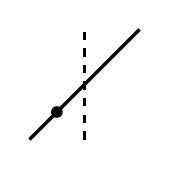
\begin{tikzpicture}[very thick,baseline,scale=.7]
  \draw(-3,0) +(-1,-1) -- +(1,1);
  \draw[dashed](-3,0) +(0,-1) -- +(0,1);
\fill (-3.5,-.5) circle (3pt); \end{tikzpicture}
=
 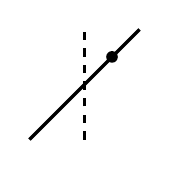
\begin{tikzpicture}[very thick,baseline,scale=.7] \draw(1,0) +(-1,-1) -- +(1,1);
  \draw[dashed](1,0) +(0,-1) -- +(0,1);
\fill (1.5,.5) circle (3pt);
    \end{tikzpicture} -h  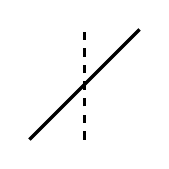
\begin{tikzpicture}[very thick,baseline,scale=.7] \draw(1,0) +(-1,-1) -- +(1,1);
  \draw[dashed](1,0) +(0,-1) -- +(0,1);
    \end{tikzpicture}
\qquad \qquad     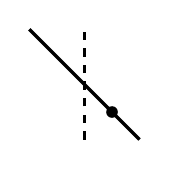
\begin{tikzpicture}[very thick,baseline,scale=.7]
  \draw(-3,0) +(1,-1) -- +(-1,1);
  \draw[dashed](-3,0) +(0,-1) -- +(0,1);
\fill (-2.5,-.5) circle (3pt); \end{tikzpicture}
=
 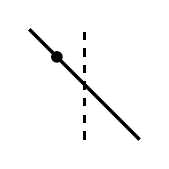
\begin{tikzpicture}[very thick,baseline,scale=.7] \draw(1,0) +(1,-1) -- +(-1,1);
  \draw[dashed](1,0) +(0,-1) -- +(0,1);
\fill (.5,.5) circle (3pt);
    \end{tikzpicture} +h  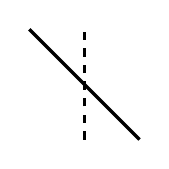
\begin{tikzpicture}[very thick,baseline,scale=.7] \draw(1,0) +(1,-1) -- +(-1,1);
  \draw[dashed](1,0) +(0,-1) -- +(0,1);
    \end{tikzpicture}
  \end{equation*}
 \begin{equation*}\subeqn\label{x-cost}
  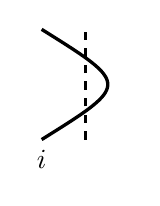
\begin{tikzpicture}[very thick,baseline,scale=.7]
    \draw (-2.8,0)  +(0,-1) .. controls (-1.2,0) ..  +(0,1) node[below,at start]{$i$};
       \draw[dashed] (-2,0)  +(0,-1)--  +(0,1);
  \end{tikzpicture}
=   p_{i,+}\Bigg(
  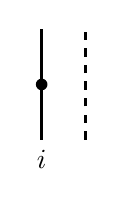
\begin{tikzpicture}[very thick,baseline,scale=.7]
 \draw[dashed] (2.3,0)  +(0,-1) -- +(0,1);
       \draw (1.5,0)  +(0,-1) -- +(0,1) node[below,at start]{$i$};
       \fill (1.5,0) circle (3pt);
\end{tikzpicture}\hspace{5mm}\Bigg)\qquad \qquad
  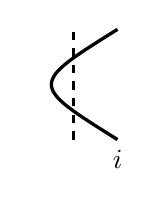
\begin{tikzpicture}[very thick,baseline,scale=.7]
          \draw[dashed] (-2,0)  +(0,-1)-- +(0,1);
  \draw (-1.2,0)  +(0,-1) .. controls (-2.8,0) ..  +(0,1) node[below,at start]{$i$};\end{tikzpicture}
           =p_{i,-}\Bigg(\hspace{5mm}
  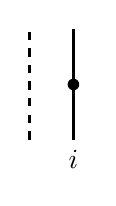
\begin{tikzpicture}[very thick,baseline,scale=.7]
    \draw (2.5,0)  +(0,-1) -- +(0,1) node[below,at start]{$i$};
       \draw[dashed] (1.7,0)  +(0,-1) -- +(0,1) ;
       \fill (2.5,0) circle (3pt);\end{tikzpicture}\Bigg)
\end{equation*}
\begin{equation*}\subeqn\label{x-triple-smart}
    \begin{tikzpicture}[very thick,scale=.9,baseline]
      \draw[postaction={decorate,decoration={markings,
    mark=at position .2 with {\arrow[scale=1.3]{<}}}}] (-3,0) +(1,-1) .. controls (-4,0) .. +(-1,1) node[below,at start]{$i$}; \draw[postaction={decorate,decoration={markings,
    mark=at position .8 with {\arrow[scale=1.3]{<}}}}]
      (-3,0) +(-1,-1) .. controls (-4,0) .. +(1,1) node[below,at start]{$i$}; \draw[dashed]
      (-3,0) +(0,-1)--  +(0,1); \node at (-1,0) {=}; \draw[postaction={decorate,decoration={markings,
    mark=at position .8 with {\arrow[scale=1.3]{<}}}}] (1,0) +(1,-1) .. controls
      (2,0) .. +(-1,1)
      node[below,at start]{$i$}; \draw[postaction={decorate,decoration={markings,
    mark=at position .2 with {\arrow[scale=1.3]{<}}}}] (1,0) +(-1,-1) .. controls
      (2,0) .. +(1,1)
      node[below,at start]{$i$}; \draw[dashed] (1,0) +(0,-1) -- +(0,1); \node at (2.8,0)
      {$+$};        \draw (6.2,0)
      +(1,-1) -- +(1,1) node[below,at start]{$i$}; \draw (6.2,0)
      +(-1,-1) -- +(-1,1) node[below,at start]{$i$}; \draw[dashed] (6.2,0)
      +(0,-1) -- +(0,1); 
\node[inner ysep=8pt,inner xsep=5pt,fill=white,draw,scale=.8] at (6.2,0){$\displaystyle \frac{p_{i,+}(y_n)-p_{i,-}(y_1)}{y_n-y_1-h}$};
    \end{tikzpicture}
  \end{equation*}
\begin{equation*}\subeqn\label{x-triple-dumb}
    \begin{tikzpicture}[very thick,scale=.9,baseline]
      \draw[postaction={decorate,decoration={markings,
    mark=at position .2 with {\arrow[scale=1.3]{<}}}}] (-3,0) +(1,-1) .. controls (-4,0) .. +(-1,1) node[below,at start]{$j$}; \draw[postaction={decorate,decoration={markings,
    mark=at position .8 with {\arrow[scale=1.3]{<}}}}]
      (-3,0) +(-1,-1) .. controls (-4,0) .. +(1,1) node[below,at start]{$i$}; \draw[dashed]
      (-3,0) +(0,-1)--  +(0,1); \node at (-1,0) {=}; \draw[postaction={decorate,decoration={markings,
    mark=at position .8 with {\arrow[scale=1.3]{<}}}}] (1,0) +(1,-1) .. controls
      (2,0) .. +(-1,1)
      node[below,at start]{$j$}; \draw[postaction={decorate,decoration={markings,
    mark=at position .2 with {\arrow[scale=1.3]{<}}}}] (1,0) +(-1,-1) .. controls
      (2,0) .. +(1,1)
      node[below,at start]{$i$}; \draw[dashed] (1,0) +(0,-1) -- +(0,1); 
    \end{tikzpicture}
\qquad \text{if $i\neq j$.}
  \end{equation*}
  \begin{equation*}\subeqn\label{x-triple-extra-dumb}
    \begin{tikzpicture}[very thick,scale=.9,baseline]
      \draw[postaction={decorate,decoration={markings,
    mark=at position .4 with {\arrow[scale=1.3]{<}}}}] (-3,0) +(-1,-1) to[out=90,in=-150] node[below,at start]{$j$} +(1,1) ; \draw[postaction={decorate,decoration={markings,
    mark=at position .8 with {\arrow[scale=1.3]{<}}}}]
      (-3,0) +(-2,-1) -- +(2,1) node[below,at start]{$i$}; \draw[dashed]
      (-3,0) +(0,-1)--  +(0,1); \node at (-1,0) {=}; \draw[postaction={decorate,decoration={markings,
    mark=at position .6 with {\arrow[scale=1.3]{<}}}}] (1,0) +(-1,-1) to [out=30,in=-90] node[below,at start]{$j$} +(1,1)
      ; \draw[postaction={decorate,decoration={markings,
    mark=at position .2 with {\arrow[scale=1.3]{<}}}}]
      (1,0) +(-2,-1) -- +(2,1) node[below,at start]{$i$}; \draw[dashed] (1,0) +(0,-1) -- +(0,1); 
    \end{tikzpicture}
  \end{equation*}

  \end{itemize}

  We let the {\bf cylindrical BFN category} be the category whose objects are subsets of $(\R/\Z)\setminus \{0\}$, with each element of the subset labeled with $i\in \Gamma$, and whose morphisms are cylindrical KLR diagrams with the source at bottom and target at top.  
\end{definition}

We wish to compare this with the extended BFN category discussed above.  For the sake of notation.  We let $z_{i,k}$ for $k=1,\dots, v_i$ denote the weights of $\C^{v_i}$ as a module over
$GL(v_i)$.  Consider the set of elements of $\ft_{\R}\subset \oplus_i \mathfrak{gl}(v_i)$ for which $z_{i,k}\not\in \Z $ and  $z_{i,k}-z_{j,m}\not\in \Z$ unless $i=j$ and $k=m$; note that this is implied by genericity for $i=j$ (due to the need to avoid translates of root hyperplanes) or when $i$ and $j$ are joined by an edge (to avoid translates of weight hyperplanes), but for simplicity, we require it for all pairs of nodes.
For each such element of $\ft_{\R}$, we define an object of the cylindrical BFN category by taking the subset of $\R/\Z$ to be the residues $z_{i,k}\pmod \Z$, each labeled with the node $i$.  Our assumptions imply that these avoid $x=0$ and each other.  

Note that this object is unchanged up to isomorphism if we deform our element in $\ft_{\R}$ without changing our desired conditions.  Furthermore, the action of the affine Weyl group leaves this subset with labeling unchanged; in fact, two elements of $\ft_{\R}$ give the same object if and only if they are conjugate under the action of the affine Weyl group.  

The claim we wish to prove is that there is an equivalence between the extended and cylindrical BFN categories; of course, the cylindrical BFN category is constructed specifically to make this theorem work.  The most important morphisms in the extended BFN category can be thought of as associated to a path from one chamber to another; we can visualize these paths as cylindrical diagrams, where the slice of the cylinder at $y=t$ is the residues mod $\Z$ of the position of the path at time $t$. 
Making this precise requires a bit more care about notation.
First, we invert the map sending an element of $\ft_{\R}$ to its residues.  For a given $\Bi$, 
we let $n_{i,k}$ be the $k$th integer in $[1,n]$ such that
$i_{n_{i,k}}=i$ (in increasing order).    We let $\tau_{i,k}$ be the dual coweight to $z_{i,k}$, thought of as an
element of the extended affine Weyl group, and let $\rho_i$ be the element of the  affine Weyl group that acts by 
\begin{equation*}
    \rho_i(z_{j,k})=\begin{cases}
    z_{j,k} & i\neq j\\
    z_{i,k-1} & i=j, k\neq 1\\
    z_{i,v_i}+1 & i=j,k=1
    \end{cases}
\end{equation*}

Given $\Bi$, consider the element $\xi_{\Bi}\in \ft\subset \oplus_i \mathfrak{gl}(v_i)$ where $z_{i,k}=n_{i,k}/n$; that is, its component in $\mathfrak{gl}(v_i)$ is the diagonal matrix $\operatorname{diag}(n_{i,1}/(n+1),\dots, n_{i,v_i}/(n+1))$.  Obviously, if we take residues in $\R/\Z$, this returns the object in the cylindrical BFN category with labels $\Bi$.

\begin{proposition}
  There is a natural functor from the cylindrical BFN category 
to the extended BFN
  $\mathscr{B}$ category with $\epsilon=0$, sending $(i_1,\dots, i_n)$ to the chamber  containing
  the point $\xi_{\Bi}$, and sending
  \begin{itemize}
  \item a dot on the $n_{i,k}$th strand to the weight $z_{i,k}$
  \item the crossing of the $p$th and $(p+1)$-st strands to
    $r(\xi_{s_p\cdot \Bi},\xi_{\Bi})$ for if $i_p\neq i_{p+1}$ and
    $p\in [1,n-1]$.
\item the crossing of the $p$th and $(p+1)$-st strands to
    $s_pu_i$ for if $i_p= i_{p+1}$ and $p\in [1,n-1]$.
\item the rightward crossing of a strand with label $i$ over $x=0$ to
  $y_{\rho_i}^{-1}r(\xi_{\rho\cdot \Bi}+\tau_{i,1},\xi_{\Bi})$, and the
  leftward to $y_{\rho_i}r(\xi_{\rho^{-1}\cdot \Bi}-\tau_{i,v_i},\xi_{\Bi})$.
  \end{itemize}
\end{proposition}
Let us give a simple example.  Consider the running example of \cite{WebSD}: $G=GL(2)$ and $V\cong \C^2\oplus \C^2$.  We have a natural isomorphism $\ft_{\R}\cong \R^2$ with the coordinates given by $z_{1},z_{2}$.  The hyperplanes we wish to avoid are when $z_1\in \Z,z_2\in \Z$ or $z_1-z_2\in \Z$.  There is only one object up to isomorphism in the BFN category, and the corresponding $\xi$ is given by $(1/3,2/3)$.  We can draw a path connecting chambers, and obtain the corresponding element $\tilde{r}$ associated to this path, using $r(\eta,\eta')$ to move across weight hyperplanes, and applying $u_\al$ whenever we cross a root hyperplane.  Note the extended affine Weyl group acts simply transitively the chambers of this arrangement, so we can visualize the endomorphisms of a single chamber by drawing and paths, and then leaving implicit that we return to our fixed chamber using the affine Weyl group.  

With these conventions, we match morphisms of the extended category to those of the cylindrical category via:
\begin{equation*} 
       \tikz[very thick,scale=.8,baseline]{
\draw (1.2,2.5)-- (1.2,-2.5) node[at start,above,scale=.8]{$z_1=1$}; \draw (-1.2,2.5)--
(-1.2,-2.5) node[at start,above,scale=.8]{$z_1=0$};
\draw (2.5,1.2)-- (-2.5,1.2) node[at start,right,scale=.8]{$z_2=1$}; \draw (2.5,-1.2)--
(-2.5,-1.2) node[at start,right,scale=.8]{$z_2=0$}; 
 \draw[dotted] (-2.5,-2.5) -- node[above right,at
        end,scale=.8]{$\alpha=0$}(2.5,2.5); 
 \draw[dotted] (-2.5,-.1) -- node[above ,at
        end,scale=.8]{$\alpha=-1$}(.1,2.5); 
 \draw[dotted] (-.1,-2.5) -- node[right,at
        end,scale=.8]{$\alpha=1$}(2.5,.1); 
\draw[->,dashed] (-.4,.4) to (.4,-.4);
}\qquad \leftrightarrow \qquad
       \tikz[very thick,xscale=1.5,baseline]{
          \draw[fringe] (-1,-1)-- (-1,1);
          \draw[fringe] (1,1)-- (1,-1);
           \draw (.4 ,-1) to (-.4,1);
        \draw (-.4 ,-1) to (.4,1);

        }
\end{equation*}
\begin{equation*} 
       \tikz[very thick,scale=.8,baseline]{
\draw (1.2,2.5)-- (1.2,-2.5) node[at start,above,scale=.8]{$z_1=1$}; \draw (-1.2,2.5)--
(-1.2,-2.5) node[at start,above,scale=.8]{$z_1=0$};
\draw (2.5,1.2)-- (-2.5,1.2) node[at start,right,scale=.8]{$z_2=1$}; \draw (2.5,-1.2)--
(-2.5,-1.2) node[at start,right,scale=.8]{$z_2=0$}; 
 \draw[dotted] (-2.5,-2.5) -- node[above right,at
        end,scale=.8]{$\alpha=0$}(2.5,2.5); 
 \draw[dotted] (-2.5,-.1) -- node[above ,at
        end,scale=.8]{$\alpha=-1$}(.1,2.5); 
 \draw[dotted] (-.1,-2.5) -- node[right,at
        end,scale=.8]{$\alpha=1$}(2.5,.1); 
\draw[->,dashed] (-.4,.4) to (.4,2);
}\qquad \leftrightarrow \qquad
       \tikz[very thick,xscale=1.5,baseline]{
          \draw[fringe] (-1,-1)-- (-1,1);
          \draw[fringe] (1,1)-- (1,-1);
           \draw (.4 ,-1) to (1,0);
           \draw (-1,0) to(-.4,1);
        \draw (-.4 ,-1) to (.4,1);

        }
\end{equation*}
\begin{equation*} 
       \tikz[very thick,scale=.8,baseline]{
\draw (1.2,2.5)-- (1.2,-2.5) node[at start,above,scale=.8]{$z_1=1$}; \draw (-1.2,2.5)--
(-1.2,-2.5) node[at start,above,scale=.8]{$z_1=0$};
\draw (2.5,1.2)-- (-2.5,1.2) node[at start,right,scale=.8]{$z_2=1$}; \draw (2.5,-1.2)--
(-2.5,-1.2) node[at start,right,scale=.8]{$z_2=0$}; 
 \draw[dotted] (-2.5,-2.5) -- node[above right,at
        end,scale=.8]{$\alpha=0$}(2.5,2.5); 
 \draw[dotted] (-2.5,-.1) -- node[above ,at
        end,scale=.8]{$\alpha=-1$}(.1,2.5); 
 \draw[dotted] (-.1,-2.5) -- node[right,at
        end,scale=.8]{$\alpha=1$}(2.5,.1); 
\draw[->,dashed] (-.4,.4) to (-2,-.4);
}\qquad \leftrightarrow \qquad
       \tikz[very thick,xscale=1.5,baseline]{
          \draw[fringe] (-1,-1)-- (-1,1);
          \draw[fringe] (1,1)-- (1,-1);
           \draw (.4 ,1) to (1,0);
           \draw (-1,0) to(-.4,-1);
        \draw (-.4 ,1) to (.4,-1);

        }
\end{equation*}


\begin{proof}
  This is clear from comparing the relations
  (\ref{b-first-QH}--\ref{x-triple-dumb}) with those of the extended
  BFN category.
  
  In particular, \begin{itemize}
      \item The relations (\ref{b-first-QH}--\ref{b-second-QH}) together with isotopy of dots past the $y$-value of crossings on differently labeled strands match precisely \cite[(3.1e)]{WebSD}.
            \item The relation (\ref{dot-slide}) follows from combining \cite[(3.1e)\& (3.2c)]{WebSD} 
      \item  The relations (\ref{b-nilHecke-1}--\ref{b-nilHecke-2}) and isotopy of dots past the $y$-value of crossings on like labeled strands matches \cite[(3.4d)]{WebSD}.

      \item The usual isotopy of diagrams follows from applications of \cite[(3.1d) \& (3.4e)]{WebSD} in cases where they are boring (there are no correction terms).  This also covers (\ref{b-triple-dumb},\ref{x-triple-dumb}--\ref{x-triple-extra-dumb}) in the cases where no two strands have the same label.
      \item The first relation of (\ref{b-black-bigon}) is \cite[(3.4a)]{WebSD}.
      \item The second relation of (\ref{b-black-bigon}) is \cite[(3.1d)]{WebSD} in the special case where we cross one of the hyperplanes for $z_{i,k}-z_{j,m}$ twice.
         \item The relation (\ref{x-cost}) is another application of \cite[(3.1d)]{WebSD}, but in the case of hyperplanes for $z_{i,k}$.  
      \item The relations (\ref{b-triple-dumb}--\ref{b-triple-smart}, \ref{x-triple-smart}--\ref{x-triple-extra-dumb}) match \cite[(3.4e)]{WebSD} for the two different types of weight hyperplanes.
  \end{itemize}
  This confirms the full list of relations and thus proves the theorem.
\end{proof}
We can also naturally study the weight modules over the extended category in
this framework.  We have a category $\widehat{\BFN}$ whose objects are sequences $\Bi$
and weights $(a_1,\cdots,a_n)$ that give generalized eigenvalues of
the dots in $\K$, with morphisms $(\Bi,\Ba)\to (\Bj,\Bb)$  given by
the coarsest completion of $e(\Bi)\BFN e(\Bj)$ where $y_k$ acts on the
left with generalized eigenvalue $a_k$ and on the right with
generalized eigenvalue $b_k$.  As in \cite{WebSD}, finite dimensional representations of
the category $\widehat{\BFN}$ are equivalent to weight representations of $\BFN$.

Pick an order on $\Gamma$, and number the vertices $1,\dots, r$; for
simplicity, we orient the edges in the increasing direction. Let $\Bi$
be the sequence where the labels are in increasing order.  Let $e_0$
be the idempotent endomorphism of this sequence where we multiply each
group of strands with the same label with a primitive idempotent in
the nilHecke algebra.
If we take $b_e=-\nicefrac{a_{ij}}{2}-p$ for $p=1,\dots, -a_{ij}$ for
the $a_{ij}$ edges joining $i$ and $j$, then \cite[Thm. B.18]{BFNplus} shows that:
\begin{proposition}
The endomorphisms of $e_0$ are isomorphic to the truncated shifted
Yangian for $\Gamma$.  
\end{proposition}
Thus, this category is another framework in which to view the Yangian,
and there is a natural quotient functor from weight modules over
$\BFN$ to those of the Yangian, given by multiplication by $e_0$.    We'll develop this further in \cite{KTWWY2} to better understand the representation theory of Yangians. 



\subsection{Cylindrical KLR algebras}
\label{sec:definition}

 
 In the characteristic 0 case, for the Coulomb branch of a quiver gauge theory, we can describe the category of weight modules over $\EuScript{A}$ in terms of weighted KLR algebras (\cite[\S 4.4]{WebSD}).  The category $\pStein_\K$ which appears in characteristic $p$ can be described in similar terms, but ones which seem not to have been deeply studied in the literature.  
 
 Fix a quiver $\Gamma$, and $\ell$-tuples $(\theta_1,\dots, \theta_\ell)\in (\R/\Z)^{\ell},$ and $(\la_1, \dots, \la_\ell)$ of dominant weights for $\fg_\Gamma$.  For simplicity, we'll assume that $(0,\theta_1,\dots, \theta_\ell)$ are cyclically ordered.   On the cylinder $\R/\Z\times [0,1]$, we'll draw in red lines at $x=\theta_i$.  
 \begin{definition}\label{def:cyl-Stendhal}
  A {\bf cylindrical Stendhal diagram} is a collection of finitely many
  oriented curves in $\R/\Z\times [0,1]$ (which are all colored
  black). Each curve is labeled with $i\in \Gamma$ and decorated with
  finitely many dots.  The diagram must be locally of the
  form \begin{equation*}
\begin{tikzpicture}
  \draw[very thick,postaction={decorate,decoration={markings,
    mark=at position .75 with {\arrow[scale=1.3]{<}}}}] (-4,0) +(-1,-1) -- +(1,1);
   % node[below,at start] {$i$};
  \draw[very thick,postaction={decorate,decoration={markings,
    mark=at position .75 with {\arrow[scale=1.3]{<}}}}](-4,0) +(1,-1) -- +(-1,1);
  %  node[below,at start] {$j$};

%\draw[very thick] (0,0) +(0,-1) -- +(0,1)
%node[below, at start]{$i$};
%\fill (0,0) circle (5pt);


  \draw[very thick,postaction={decorate,decoration={markings,
    mark=at position .75 with {\arrow[scale=1.3]{<}}}}](-1,0) +(0,-1) --  node
  [midway,circle,fill=black,inner sep=2pt]{}
  +(0,1);
  
  \draw[very thick,postaction={decorate,decoration={markings,
    mark=at position .75 with {\arrow[scale=1.3]{<}}}}] (2,0) +(-1,-1) -- +(1,1);
   % node[below,at start] {$i$};
  \draw[very thick,wei](2,0) +(0,-1) -- +(0,1);
  
  \draw[very thick,postaction={decorate,decoration={markings,
    mark=at position .75 with {\arrow[scale=1.3]{<}}}}] (5,0) +(1,-1) -- +(-1,1);
   % node[below,at start] {$i$};
  \draw[very thick,wei](5,0) +(0,-1) -- +(0,1);
\end{tikzpicture}
\end{equation*}
with each curve oriented in the negative direction.  The curves must
meet the circles at
$y=0$ and $y=1$ at distinct points with $x\neq 0$. We consider these
up to isotopy preserving the conditions above.  
\end{definition}
 
 We'll draw these on the page in the rectangle $[0,1]\times [0,1]$ with seams on the left and right side of the diagram where we should glue to obtain the cylindrical diagram.  An example of such a diagram is \begin{equation*} 
       \tikz[very thick,xscale=1.5]{
          \draw[fringe] (-1,-1)-- (-1,1);
          \draw[fringe] (1,1)-- (1,-1);
          \draw[wei] (-.8,-1)--node[below, at start ]{$\la$} (-.8,1);
          \draw[wei] (.4 ,-1)--node[below, at start ]{$\mu$} (.4,1);
\draw (-1,.2) to[out=30,in=-90] node[above, at end]{$i$} (.2,1);
           \draw (.6 ,-1) to[out=90,in=-150] node[below, at start ]{$i$}(1,.2);
           \draw (-1,-.2) to[out=-30,in=90]node[below, at end ]{$k$} (-.5,-1);
           \draw (-.2 ,1) to[out=-90,in=150] node[midway,circle,fill=black,inner sep=2pt]{} node[above, at start ]{$k$}(1,-.2);
           \draw (-.2,-1) to[out=90,in=-90] node[below, at start ]{$i$} node[above, at end]{$i$} (-.5,1);
        }
\end{equation*}
 
We can multiply these in the usual manner, stacking the diagrams and using an isotopy to match the top of one diagram with the bottom of the other. 

\begin{definition}  The {\bf cylindrical KLR algebra} attached to these data is the quotient of the formal span of Stendhal diagrams 
 by the following local relations:
 \begin{itemize}
  \item we have the usual KLR relations for the polynomials $Q_{ij}=(u-v)^{\# j\to i}(v-u)^{\# i\to j}$:
  \newseq
%\begin{figure}[h!]
\begin{equation*}\subeqn\label{first-QH}
    \begin{tikzpicture}[scale=.9,baseline]
      \draw[very thick,postaction={decorate,decoration={markings,
    mark=at position .2 with {\arrow[scale=1.3]{<}}}}](-4,0) +(-1,-1) -- +(1,1) node[below,at start]
      {$i$}; \draw[very thick,postaction={decorate,decoration={markings,
    mark=at position .2 with {\arrow[scale=1.3]{<}}}}](-4,0) +(1,-1) -- +(-1,1) node[below,at
      start] {$j$}; \fill (-4.5,.5) circle (3pt);
      % \draw[very thick] (0,0) +(0,-1) -- +(0,1) node[below, at
      % start]{$i$}; \fill (0,0) circle (5pt);
      \node at (-2,0){=}; \draw[very thick,postaction={decorate,decoration={markings,
    mark=at position .8 with {\arrow[scale=1.3]{<}}}}](0,0) +(-1,-1) -- +(1,1)
      node[below,at start] {$i$}; \draw[very thick,postaction={decorate,decoration={markings,
    mark=at position .8 with {\arrow[scale=1.3]{<}}}}](0,0) +(1,-1) --
      +(-1,1) node[below,at start] {$j$}; \fill (.5,-.5) circle (3pt);
      \node at (4,0){unless $i=j$};
    \end{tikzpicture}
  \end{equation*}
\begin{equation*}\subeqn\label{second-QH}
    \begin{tikzpicture}[scale=.9,baseline]
      \draw[very thick,postaction={decorate,decoration={markings,
    mark=at position .2 with {\arrow[scale=1.3]{<}}}}](-4,0) +(-1,-1) -- +(1,1) node[below,at start]
      {$i$}; \draw[very thick,postaction={decorate,decoration={markings,
    mark=at position .2 with {\arrow[scale=1.3]{<}}}}](-4,0) +(1,-1) -- +(-1,1) node[below,at
      start] {$j$}; \fill (-3.5,.5) circle (3pt);
      % \draw[very thick] (0,0) +(0,-1) -- +(0,1) node[below, at
      % start]{$i$}; \fill (0,0) circle (5pt);
      \node at (-2,0){=}; \draw[very thick,postaction={decorate,decoration={markings,
    mark=at position .8 with {\arrow[scale=1.3]{<}}}}](0,0) +(-1,-1) -- +(1,1)
      node[below,at start] {$i$}; \draw[very thick,postaction={decorate,decoration={markings,
    mark=at position .8 with {\arrow[scale=1.3]{<}}}}](0,0) +(1,-1) --
      +(-1,1) node[below,at start] {$j$}; \fill (-.5,-.5) circle (3pt);
      \node at (4,0){unless $i=j$};
    \end{tikzpicture}
  \end{equation*}
\begin{equation*}\subeqn\label{nilHecke-1}
    \begin{tikzpicture}[scale=.9,baseline]
      \draw[very thick,postaction={decorate,decoration={markings,
    mark=at position .2 with {\arrow[scale=1.3]{<}}}}](-4,0) +(-1,-1) -- +(1,1) node[below,at start]
      {$i$}; \draw[very thick,postaction={decorate,decoration={markings,
    mark=at position .2 with {\arrow[scale=1.3]{<}}}}](-4,0) +(1,-1) -- +(-1,1) node[below,at
      start] {$i$}; \fill (-4.5,.5) circle (3pt);
      % \draw[very thick] (0,0) +(0,-1) -- +(0,1) node[below, at
      % start]{$i$}; \fill (0,0) circle (5pt);
      \node at (-2,0){=}; \draw[very thick,postaction={decorate,decoration={markings,
    mark=at position .8 with {\arrow[scale=1.3]{<}}}}](0,0) +(-1,-1) -- +(1,1)
      node[below,at start] {$i$}; \draw[very thick,postaction={decorate,decoration={markings,
    mark=at position .8 with {\arrow[scale=1.3]{<}}}}](0,0) +(1,-1) --
      +(-1,1) node[below,at start] {$i$}; \fill (.5,-.5) circle (3pt);
      \node at (2,0){$+$}; \draw[very thick,postaction={decorate,decoration={markings,
    mark=at position .5 with {\arrow[scale=1.3]{<}}}}](4,0) +(-1,-1) -- +(-1,1)
      node[below,at start] {$i$}; \draw[very thick,postaction={decorate,decoration={markings,
    mark=at position .5 with {\arrow[scale=1.3]{<}}}}](4,0) +(0,-1) --
      +(0,1) node[below,at start] {$i$};
    \end{tikzpicture}
  \end{equation*}
 \begin{equation*}\subeqn\label{nilHecke-2}
    \begin{tikzpicture}[scale=.9,baseline]
      \draw[very thick,postaction={decorate,decoration={markings,
    mark=at position .8 with {\arrow[scale=1.3]{<}}}}](-4,0) +(-1,-1) -- +(1,1) node[below,at start]
      {$i$}; \draw[very thick,postaction={decorate,decoration={markings,
    mark=at position .8 with {\arrow[scale=1.3]{<}}}}](-4,0) +(1,-1) -- +(-1,1) node[below,at
      start] {$i$}; \fill (-4.5,-.5) circle (3pt);
      % \draw[very thick] (0,0) +(0,-1) -- +(0,1) node[below, at
      % start]{$i$}; \fill (0,0) circle (5pt);
      \node at (-2,0){=}; \draw[very thick,postaction={decorate,decoration={markings,
    mark=at position .2 with {\arrow[scale=1.3]{<}}}}](0,0) +(-1,-1) -- +(1,1)
      node[below,at start] {$i$}; \draw[very thick,postaction={decorate,decoration={markings,
    mark=at position .2 with {\arrow[scale=1.3]{<}}}}](0,0) +(1,-1) --
      +(-1,1) node[below,at start] {$i$}; \fill (.5,.5) circle (3pt);
      \node at (2,0){$+$}; \draw[very thick,postaction={decorate,decoration={markings,
    mark=at position .5 with {\arrow[scale=1.3]{<}}}}](4,0) +(-1,-1) -- +(-1,1)
      node[below,at start] {$i$}; \draw[very thick,postaction={decorate,decoration={markings,
    mark=at position .5 with {\arrow[scale=1.3]{<}}}}](4,0) +(0,-1) --
      +(0,1) node[below,at start] {$i$};
    \end{tikzpicture}
  \end{equation*}
  \begin{equation*}\subeqn\label{black-bigon}
    \begin{tikzpicture}[very thick,scale=.9,baseline]
      \draw[postaction={decorate,decoration={markings,
    mark=at position .5 with {\arrow[scale=1.3]{<}}}}] (-2.8,0) +(0,-1) .. controls (-1.2,0) ..  +(0,1)
      node[below,at start]{$i$}; \draw[postaction={decorate,decoration={markings,
    mark=at position .5 with {\arrow[scale=1.3]{<}}}}] (-1.2,0) +(0,-1) .. controls
      (-2.8,0) ..  +(0,1) node[below,at start]{$i$}; \node at (-.5,0)
      {=}; \node at (0.4,0) {$0$};
\node at (1.5,.05) {and};
    \end{tikzpicture}
\hspace{.4cm}
    \begin{tikzpicture}[very thick,scale=.9,baseline]

      \draw[postaction={decorate,decoration={markings,
    mark=at position .5 with {\arrow[scale=1.3]{<}}}}] (-2.8,0) +(0,-1) .. controls (-1.2,0) ..  +(0,1)
      node[below,at start]{$i$}; \draw[postaction={decorate,decoration={markings,
    mark=at position .5 with {\arrow[scale=1.3]{<}}}}] (-1.2,0) +(0,-1) .. controls
      (-2.8,0) ..  +(0,1) node[below,at start]{$j$}; \node at (-.5,0)
      {=}; 
\draw (1.8,0) +(0,-1) -- +(0,1) node[below,at start]{$j$};
      \draw (1,0) +(0,-1) -- +(0,1) node[below,at start]{$i$}; 
\node[inner xsep=10pt,fill=white,draw,inner ysep=8pt] at (1.4,0) {$Q_{ij}(y_1,y_2)$};
    \end{tikzpicture}
  \end{equation*}
 \begin{equation*}\subeqn\label{triple-dumb}
    \begin{tikzpicture}[very thick,scale=.9,baseline]
      \draw[postaction={decorate,decoration={markings,
    mark=at position .2 with {\arrow[scale=1.3]{<}}}}] (-3,0) +(1,-1) -- +(-1,1) node[below,at start]{$k$}; \draw[postaction={decorate,decoration={markings,
    mark=at position .8 with {\arrow[scale=1.3]{<}}}}]
      (-3,0) +(-1,-1) -- +(1,1) node[below,at start]{$i$}; \draw[postaction={decorate,decoration={markings,
    mark=at position .5 with {\arrow[scale=1.3]{<}}}}]
      (-3,0) +(0,-1) .. controls (-4,0) ..  +(0,1) node[below,at
      start]{$j$}; \node at (-1,0) {=}; \draw[postaction={decorate,decoration={markings,
    mark=at position .8 with {\arrow[scale=1.3]{<}}}}] (1,0) +(1,-1) -- +(-1,1)
      node[below,at start]{$k$}; \draw[postaction={decorate,decoration={markings,
    mark=at position .2 with {\arrow[scale=1.3]{<}}}}] (1,0) +(-1,-1) -- +(1,1)
      node[below,at start]{$i$}; \draw[postaction={decorate,decoration={markings,
    mark=at position .5 with {\arrow[scale=1.3]{<}}}}] (1,0) +(0,-1) .. controls
      (2,0) ..  +(0,1) node[below,at start]{$j$}; \node at (5,0)
      {unless $i=k\neq j$};
    \end{tikzpicture}
  \end{equation*}
\begin{equation*}\subeqn\label{triple-smart}
    \begin{tikzpicture}[very thick,scale=.9,baseline]
      \draw[postaction={decorate,decoration={markings,
    mark=at position .2 with {\arrow[scale=1.3]{<}}}}] (-3,0) +(1,-1) -- +(-1,1) node[below,at start]{$i$}; \draw[postaction={decorate,decoration={markings,
    mark=at position .8 with {\arrow[scale=1.3]{<}}}}]
      (-3,0) +(-1,-1) -- +(1,1) node[below,at start]{$i$}; \draw[postaction={decorate,decoration={markings,
    mark=at position .5 with {\arrow[scale=1.3]{<}}}}]
      (-3,0) +(0,-1) .. controls (-4,0) ..  +(0,1) node[below,at
      start]{$j$}; \node at (-1,0) {=}; \draw[postaction={decorate,decoration={markings,
    mark=at position .8 with {\arrow[scale=1.3]{<}}}}] (1,0) +(1,-1) -- +(-1,1)
      node[below,at start]{$i$}; \draw[postaction={decorate,decoration={markings,
    mark=at position .2 with {\arrow[scale=1.3]{<}}}}] (1,0) +(-1,-1) -- +(1,1)
      node[below,at start]{$i$}; \draw[postaction={decorate,decoration={markings,
    mark=at position .5 with {\arrow[scale=1.3]{<}}}}] (1,0) +(0,-1) .. controls
      (2,0) ..  +(0,1) node[below,at start]{$j$}; \node at (2.8,0)
      {$+$};        \draw (6.2,0)
      +(1,-1) -- +(1,1) node[below,at start]{$i$}; \draw (6.2,0)
      +(-1,-1) -- +(-1,1) node[below,at start]{$i$}; \draw (6.2,0)
      +(0,-1) -- +(0,1) node[below,at start]{$j$}; 
\node[inner ysep=8pt,inner xsep=5pt,fill=white,draw,scale=.8] at (6.2,0){$\displaystyle \frac{Q_{ij}(y_3,y_2)-Q_{ij}(y_1,y_2)}{y_3-y_1}$};
    \end{tikzpicture}
  \end{equation*}
  \item  The ``cost'' of a separating a red and a black line is adding $\la^i=\al_i^\vee(\la)$ dots to the black strand.
  \begin{equation}\label{cost}
  \begin{tikzpicture}[very thick,baseline=1.6cm]
    \draw (-2.8,0)  +(0,-1) .. controls (-1.2,0) ..  +(0,1) node[below,at start]{$i$};
       \draw[wei] (-1.2,0)  +(0,-1) .. controls (-2.8,0) ..  +(0,1) node[below,at start]{$\la$};
           \node at (-.3,0) {=};
    \draw[wei] (2.8,0)  +(0,-1) -- +(0,1) node[below,at start]{$\la$};
       \draw (1.2,0)  +(0,-1) -- +(0,1) node[below,at start]{$i$};
       \fill (1.2,0) circle (3pt) node[left=3pt]{$\la^i$};
          \draw[wei] (-2.8,3)  +(0,-1) .. controls (-1.2,3) ..  +(0,1) node[below,at start]{$\la$};
  \draw (-1.2,3)  +(0,-1) .. controls (-2.8,3) ..  +(0,1) node[below,at start]{$i$};
           \node at (-.3,3) {=};
    \draw (2.8,3)  +(0,-1) -- +(0,1) node[below,at start]{$i$};
       \draw[wei] (1.2,3)  +(0,-1) -- +(0,1) node[below,at start]{$\la$};
       \fill (2.8,3) circle (3pt) node[right=3pt]{$\la^i$};
  \end{tikzpicture}
\end{equation}
\item  All black crossings and dots can pass through red lines.  For the latter two
  relations (\ref{dumb}--\ref{red-dot}), we also include their mirror images:
\newseq
  \begin{equation*}\subeqn
    \begin{tikzpicture}[very thick,baseline]\label{red-triple-correction}
      \draw (-3,0)  +(1,-1) -- +(-1,1) node[at start,below]{$i$};
      \draw (-3,0) +(-1,-1) -- +(1,1)node [at start,below]{$j$};
      \draw[wei] (-3,0)  +(0,-1) .. controls (-4,0) .. node[below, at start]{$\la$}  +(0,1);
      \node at (-1,0) {=};
      \draw (1,0)  +(1,-1) -- +(-1,1) node[at start,below]{$i$};
      \draw (1,0) +(-1,-1) -- +(1,1) node [at start,below]{$j$};
      \draw[wei] (1,0) +(0,-1) .. controls (2,0) ..  node[below, at start]{$\la$} +(0,1);   
\node at (2.6,0) {$+ $};
      \draw (6.5,0)  +(1,-1) -- +(1,1) node[midway,circle,fill,inner sep=2.5pt,label=right:{$a$}]{} node[at start,below]{$i$};
      \draw (6.5,0) +(-1,-1) -- +(-1,1) node[midway,circle,fill,inner sep=2.5pt,label=left:{$b$}]{} node [at start,below]{$j$};
      \draw[wei] (6.5,0) +(0,-1) -- node[below, at start]{$\la$} +(0,1);
\node at (3.8,-.2){$\displaystyle \delta_{i,j}\sum_{a+b+1=\la^i} $}  ;
 \end{tikzpicture}
  \end{equation*}
\begin{equation*}\subeqn\label{dumb}
    \begin{tikzpicture}[very thick,baseline=2.85cm]
      \draw[wei] (-3,3)  +(1,-1) -- +(-1,1);
      \draw (-3,3)  +(0,-1) .. controls (-4,3) ..  +(0,1);
      \draw (-3,3) +(-1,-1) -- +(1,1);
      \node at (-1,3) {=};
      \draw[wei] (1,3)  +(1,-1) -- +(-1,1);
  \draw (1,3)  +(0,-1) .. controls (2,3) ..  +(0,1);
      \draw (1,3) +(-1,-1) -- +(1,1);    \end{tikzpicture}
  \end{equation*}
\begin{equation*}\subeqn\label{red-dot}
    \begin{tikzpicture}[very thick,baseline]
  \draw(-3,0) +(-1,-1) -- +(1,1);
  \draw[wei](-3,0) +(1,-1) -- +(-1,1);
\fill (-3.5,-.5) circle (3pt);
\node at (-1,0) {=};
 \draw(1,0) +(-1,-1) -- +(1,1);
  \draw[wei](1,0) +(1,-1) -- +(-1,1);
\fill (1.5,.5) circle (3pt);
    \end{tikzpicture}
  \end{equation*}
  \end{itemize}
  We let the {\bf cylindrical KLR category} be the category whose objects are subsets of $(\R/\Z)\setminus \{\theta_*\}$, with each element of the subset labeled with $i\in \Gamma$, and whose morphisms are cylindrical KLR diagrams with the source at bottom and target at top.  The algebra $\mathring{R}$ is the endomorphisms of the sum of all objects in this category (considered up to isotopy).
\end{definition}

\begin{remark}
Note that in many earlier works, such as \cite{Webmerged,WebRou}, we had an additional local relation setting a diagram to 0 if it had a black strand at far left; we will not impose this relation since it corresponds to passing category $\cO$, and here we consider all weight modules.  It's not even clear how one could interpret this relation on the circle, which matches with the fact that category $\cO$ doesn't make sense in characteristic $p$.  
\end{remark}
We fix number of black strands to be $n$.  Fix one of our red strands to be ``first'' as a reference point, and number the others in terms of increasing $x$-value. We will similarly number the black strands starting at this red strand, and as in the linear case, let $y_k$ denote a dot on the $k$th black strand, $\psi_k$ a crossing of the $k$th and $k+1$st black strands.  As in the linear case, we let $i_k$ be the label on the $k$th black strand, and let  $\kappa(j)$ denote the integer such that the $j$th red strand is between the $\kappa(j)$th and $(\kappa(j)+1)$st black strands.  Note that we have chosen our numbering so that $\kappa(1)=0$. 

Consider an infinite direct sum of polynomial rings in the variables $Y_i$, one for each choice of $\Bi, \kappa$ and an $n$-tuple of integers $(g_1,\dots, g_n)$.  The latter serve as ``odometers'' to track how strands wrap around the cylinder.  As usual, this action is defined by:
  \begin{equation*}
\begin{tikzpicture}[scale=.4,baseline]
\draw[wei] (-1,-1) -- (1,1) node[at start,below]{
$\la$} node[at end,above]{
$\la$};
\draw[very thick] (1,-1) -- (-1,1) node[at start,below]{
$i$} node[at end,above]{
$i$};
%\draw[very thick,|->] (1.5,0) -- (2.5,0);
\node at (2.7,0) {$\bullet\: f= f$ } ;
\end{tikzpicture}\qquad \qquad
\begin{tikzpicture}[scale=.4,baseline]
\draw[wei] (1,-1) -- (-1,1) node[at start,below]{
$\la$} node[at end,above]{
$\la$};
\draw[very thick] (-1,-1) -- (1,1) node[at start,below]{
$i$} node[at end,above]{
$i$};
\node at (3.7,0) {$\bullet\: f=Y_k^{\la^i}\cdot f$ } ;
\end{tikzpicture}\qquad \qquad
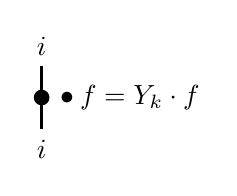
\begin{tikzpicture}[scale=.4,baseline]
\draw[very thick] (1,-1) -- (1,1) node[at start,below]{
$i$} node[at end,above]{
$i$} node[circle,midway,fill,inner sep=2pt]{};
\node at (3.8,0) {$\bullet\: f= Y_k\cdot f$ } ;
\end{tikzpicture}
  \end{equation*}
\begin{equation*}
  \begin{tikzpicture}[scale=.4]
\draw[very thick] (1,-1) -- (-1,1) node[at start,below]{
$j$} node[at end,above]{
$j$};
\draw[very thick] (-1,-1) -- (1,1) node[at start,below]{
$i$} node[at end,above]{
$i$};
\node at (7.5,0) {$\bullet\: f=\begin{cases}
 P_{ji}(Y_k,Y_{k+1}) f^{s_k} & i\neq j\\
 \displaystyle \frac{f^{s^k}- f}{Y_{k+1}-Y_{k}} & i=j  
\end{cases}$ } ;
\end{tikzpicture}
\end{equation*}
The only subtlety is that when a black strand crosses leftward over the first red strand, it goes from first to last and we must cyclically permute the variables $Y_*$ and labels $i_*$ as well as the odometer with a shift; it becomes $(g_2,\dots, g_n,g_1-1)$.  Crossing the other direction reverses this process, as well as multiplying by the required power of $Y_1$.  

The use of the ``odometer'' is a bit annoying, but necessary, since otherwise, this action would not be faithful. For example, the diagram that wraps all strands one step around the cylinder would simply match multiplication by a polynomial; in our representation, these act differently, since the former diagram increases the odometer of each strand, while the latter leaves it unchanged. 

We leave to the reader the proof of the following Lemma (the proof is an obvious port of that of \cite[Prop. 4.16]{Webmerged}, which is in turn an application of standard techniques):
\begin{lemma}\label{lem:cyl-basis}
The Hom space between two objects in the cylindrical KLR category is a free module for the left action of polynomials in the dots, with one basis vectors for each affine permutation matching the two objects, i.e. each bijection between the terminals on the top and bottom, together with choice of the number of times each strand wraps around the cylinder.  The basis vectors are given by a dotless diagram with a minimal number of crossings tracing out the chosen affine permutation.
\end{lemma}


\excise{ Consider an infinite family of variables $Y_i$ for $i\in \Z$.  We will define a representation of our category that sends each idempotent to a ring $S$ defined to be finite formal sums of formal (possibly infinite) products of polynomials such that for any finite set of variables, only finitely many terms in the product use any variable from this finite set.    This is well-defined as a ring since the multiplying two such products gives a product of the same form.

The action of diagrams is very closely related to the usual representation of the linear version of this algebra
  Choose
polynomials $P_{ij}(u,v)$ such that $Q_{ij}(u,v)=P_{ij}(u,v)P_{ji}(v,u)$.
\begin{lemma}\label{action}
  The cylindrical KLR category on $n$ black strands acts on $S$ by the rule that:
  \begin{itemize}
  \item The dots $y_m$ act as multiplication by the infinite monomial $\displaystyle\prod_{p\equiv m\pmod n}Y_p$.
  \item $e(\Bi,\kappa)\cdot \varepsilon (\Bi',\kappa')=\delta_{\Bi,\Bi'}\delta_{\kappa,\kappa'}\varepsilon(\Bi,\kappa).$
 \item Assume $\kappa(j)=k$ and $j\neq 1$. The diagram crossing the $k$th black
    strand right over the $j$th red strand sends \[f(\dots, Y_{-1},Y_0,Y_{1},\dots) \varepsilon (\Bi,\kappa)\mapsto
    f \displaystyle\prod_{p\equiv k\pmod n} Y_{p}^{\la_j^{i_k}}\varepsilon (\Bi,\kappa')\] where $\kappa'(m)=\kappa(m)-\delta_{j,m}$.  If $j=1$, then \[f(\dots, Y_{-1},Y_0,Y_{1},\dots) \varepsilon (\Bi,\kappa)\mapsto
    f(\dots, Y_{0},Y_1,Y_{2},\dots) \displaystyle\prod_{m\equiv 1\pmod n} Y_{m}^{\la_1^{i_k}}\varepsilon (\Bi,\kappa')\] where $\kappa'(m)=\kappa(m)+1-\delta_{0,m}$; that is, we shift all the variables (since we we have reindexed the numbering on black strands).
\item Assume $\kappa(j)=k$. The diagram crossing the $k+1$st black strand left of the $j$th
  red sends $\varepsilon (\Bi,\kappa)\mapsto \varepsilon (\Bi,\kappa'')$ where $\kappa''(m)=\kappa(m)+\delta_{j,m}$ if $j\neq 0$, and $\kappa''(m)=\kappa(m)-1+\delta_{j,m}$ if $j=0$.
\item Crossing the $m$th and $m+1$st black strands (assuming there is
  no red between them) sends \[f \varepsilon (\Bi,\kappa)\mapsto \begin{cases}\displaystyle \left(\prod_{p\equiv m\pmod n}\partial_p\right)f \varepsilon
  (s_m\cdot \Bi,\kappa)& i_m=i_{m+1}\\\displaystyle
 \left(\prod_{p\equiv m\pmod n} P_{ji}(Y_p,Y_{p+1})\right)f \varepsilon
  (s_m\cdot \Bi,\kappa)&i_m\neq
  i_{m+1}.\end{cases}\]  
  Some comment is needed about why the infinite product of Demazure operators is well-defined. 
\item Since the elements $\varepsilon (\Bi,\kappa)$ generate $\cP_n$
  over the polynomial ring $\C[Y_i]$, the action on any other element
  can be computed using the relations 
  past $y_i$'s.  
  \end{itemize}
More schematically, if we leave all but the two strands after the $k-1$st
black out of the diagram, we can represent this action by:
  \begin{equation*}
\begin{tikzpicture}[scale=.4,baseline]
\draw[wei] (-1,-1) -- (1,1) node[at start,below]{
$\la$} node[at end,above]{
$\la$};
\draw[very thick] (1,-1) -- (-1,1) node[at start,below]{
$i$} node[at end,above]{
$i$};
%\draw[very thick,|->] (1.5,0) -- (2.5,0);
\node at (2.7,0) {$\bullet\: f= f$ } ;
\end{tikzpicture}\qquad \qquad
\begin{tikzpicture}[scale=.4,baseline]
\draw[wei] (1,-1) -- (-1,1) node[at start,below]{
$\la$} node[at end,above]{
$\la$};
\draw[very thick] (-1,-1) -- (1,1) node[at start,below]{
$i$} node[at end,above]{
$i$};
\node at (3.7,0) {$\bullet\: f=Y_k^{\la^i}\cdot f$ } ;
\end{tikzpicture}\qquad \qquad
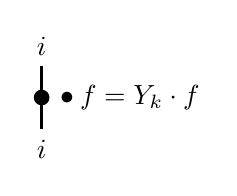
\begin{tikzpicture}[scale=.4,baseline]
\draw[very thick] (1,-1) -- (1,1) node[at start,below]{
$i$} node[at end,above]{
$i$} node[circle,midway,fill,inner sep=2pt]{};
\node at (3.8,0) {$\bullet\: f= Y_k\cdot f$ } ;
\end{tikzpicture}
  \end{equation*}
\begin{equation*}
  \begin{tikzpicture}[scale=.4]
\draw[very thick] (1,-1) -- (-1,1) node[at start,below]{
$j$} node[at end,above]{
$j$};
\draw[very thick] (-1,-1) -- (1,1) node[at start,below]{
$i$} node[at end,above]{
$i$};
\node at (7.5,0) {$\bullet\: f=\begin{cases}
 P_{ji}(Y_k,Y_{k+1}) f^{s_k} & i\neq j\\
 \displaystyle \frac{f^{s^k}- f}{Y_{k+1}-Y_{k}} & i=j  
\end{cases}$ } ;
\end{tikzpicture}
\end{equation*}
\end{lemma}}



Given a choice of $\phi$ corresponding to an element of $\fg_{\Bw}$, we let $\phi_{i,1},\dots, \phi_{i,w_i}$ be the eigenvalues of this element acting on $W_i$; for simplicity, we assume these are all integral.  We let $\ell$ be the number of distinct values of $\phi_{i,k}$ for all $i$ and $k$, and choose a numbering of these values. If $\phi_{i,k}$ is the $m$th such value,  we let $\theta_m=\frac{\phi_{i,k}+\nicefrac{1}{2}}{p}$. For simplicity, we assume that our quiver $\Gamma$ has no oriented cycles, so there is an order on vertices such that arrows always point in the increasing direction.  We call an object in the cylindrical KLR category $\boldsymbol{\theta}$-compatible if it can be isotoped to have $x$-values in the regions $[a/p,a/p+\delta]$ for $a\in \Z/p\Z$ and $\delta>0$ arbitrarily small, with the labels on strands in this region weakly increasing from left to right in each of these regions. 

Recall that for us, a choice of weight $\beta\in \ft_{1,\Fp}$ is choosing a $\beta_{i,k}\in \Fp$ for each $i\in \Gamma$ and $k\in [1,v_i]$; the corresponding element of $\ft_{1,\Fp}\subset \fg_{\Bv}\oplus \fg_{\Bw}$ has component in $\mathfrak{gl}(v_i)$ defined by $\operatorname{diag}(\beta_{i,1},\dots \beta_{i,v_i})$, and $\mathfrak{gl}(w_i)$ by $\operatorname{diag}(\phi_{i,1},\dots, \phi_{i,w_i})$.
Thus, note that $ \frac{\beta_{i,k}}{p}\in \R/\Z$ is well-defined. 
\begin{theorem}\label{thm:KLR-equiv}
The category $\pStein_\Fp$ is equivalent to the subcategory of
$\boldsymbol{\theta}$-compatible objects in the cylindrical KLR category, sending a weight $\beta$ to the object where a black strand with label $i$ is placed in the region $[\beta_{i,k},\beta_{i,k}+\delta]$ for each $i\in \Gamma, k\in [1,v_i]$, with the strands in each of these regions ordered in increasing order.
\end{theorem}
\begin{proof}
First we must describe the image of generators under this functor. \begin{itemize}
\item The weight $\varepsilon_{i,k}$ of action on the $k$th basis vector in $\C^{v_i}$ is sent to the action of the dot on the associated strand.
\item If $s_{i,k}\cdot \beta=\beta$, then we have $\beta_{i,k}=\beta_{i,k+1}$, so the corresponding strands are adjacent, and we send $\psi_{i,k}$ to the crossing of these strands with the same label.
\item The action of elements of the affine Weyl group only reorders the strands in one neighborhood of $[\beta_{i,k}/p,\beta_{i,k}/p+\delta]$ that have the same label; we do this using the ``neutral crossing'' $\al_{i,k}\psi_{i,k}+1$
\item Using the elements of the affine Weyl group, we have reduce to describing the image of $\wall(\beta,\beta')$ with the two endpoints in the same Weyl alcove.  In this case, we simply draw the straightline diagram such that the strand associated to $(i,k)$ changes $x$-value by $(\beta_i-\beta_i')/p$; this never crosses two strands with the same label, since we never change alcove.  The elements $\wall(\beta,\beta')$ that do change alcoves just have to use the ``neutral crossing'' $\al_{i,k}\psi_{i,k}+1$ when we change alcoves. 
\end{itemize} 
That this matches the representation (\ref{Y-action})  is a straight forward calculation in the usual mold.  It's worth noting that the weights of the representation that appear are either of the form $\varepsilon_{i,k}$ or $\varepsilon_{i,k}-\varepsilon_{j,m}$ if there is an edge $j\to i$.  The multiplication by the former in \ref{Y-action} is accounted for by red/black crossings and (\ref{cost}), and by the latter by black/black crossings and (\ref{black-bigon}).  This gives a functor from the $\boldsymbol{\theta}$-compatible objects to  $\pStein_\Fp$ which is easily seen to be full.  We this is an equivalence comparing the usual basis $w\tilde{r}(w^{-1}\eta',\eta)$ of morphisms in $\pStein_\Fp$ with that of Lemma \ref{lem:cyl-basis}.
\end{proof}
Implicitly, this tells us that we have an equivalence between the
representation category $\widehat{\BFN}$ for $\Fp$ and the
$\boldsymbol{\theta}$-compatible objects in the cylindrical KLR
category.  We send the sequence $\Bi$ and eigenvalues $\Ba$ to placing
elements with label $i_k$ at $a_k/p+k\delta/n$.  We map the diagrams
to the usual ones suggested by the polynomial representations.
%\begin{equation*}
%  y_k\mapsto y_k+a_k\qquad 
%\end{equation*}




\begin{example}\label{example:NZ}
Consider the case where $G=\C^*$ acting on $\C^2$ by scalars.  In this case, the Coulomb branch is $T^*\mathbb{P}^1$.  The corresponding cylindrical KLR algebra has two red strands, and one black strand, all with the same label. 
There are two idempotents in this algebra, corresponding to the two cyclic orders of the 3 strands.  
\begin{equation*}
        \tikz[xscale=.9]{
      \node[label=below:{$ x$}] at (-4.5,0){ 
       \tikz[very thick,xscale=1]{
          \draw[fringe] (-.7,-.5)-- (-.7,.5);
          \draw[fringe] (1.7,.5)-- (1.7,-.5);
          \draw[wei] (.3,-.5)-- (.3,.5);
          \draw[wei] (1.5 ,-.5)-- (1.5,.5);
\draw (-.7,0) to[out=0,in=-90] (-.2,.5);
           \draw (.9 ,-.5) to[out=90,in=180] (1.7,0);
        }
      };
      \node[label=below:{$ x^*$}] at (0,0){ 
       \tikz[very thick,xscale=1, yscale=-1]{          
       \draw[fringe] (-.7,.5)-- (-.7,-.5);
          \draw[fringe] (1.7,-.5)-- (1.7,.5);
          \draw[wei] (.3,-.5)-- (.3,.5);
          \draw[wei] (1.5 ,-.5)-- (1.5,.5);
\draw (-.7,0) to[out=0,in=-90] (-.2,.5);
           \draw (.9 ,-.5) to[out=90,in=180] (1.7,0);
        }
      };
       \node[label=below:{$ y $}] at (4.5,0){ 
        \tikz[very thick,xscale=1]{
          \draw[fringe] (-.7,-.5)-- (-.7,.5);
          \draw[fringe] (1.7,.5)-- (1.7,-.5);
          \draw[wei] (.3,-.5)-- (.3,.5);
          \draw[wei] (1.5 ,-.5)-- (1.5,.5);
\draw (.9 ,-.5)  to[out=90,in=-90] (-.2,.5);
       }
      };
      \node[label=below:{$ y^* $}] at (9,0){ 
        \tikz[very thick,xscale=1, yscale=-1]{
           \draw[fringe] (-.7,.5)-- (-.7,-.5);
          \draw[fringe] (1.7,-.5)-- (1.7,.5);
          \draw[wei] (.3,-.5)-- (.3,.5);
          \draw[wei] (1.5 ,-.5)-- (1.5,.5);
\draw (.9 ,-.5)  to[out=90,in=-90] (-.2,.5);
       }
      };
      }
\end{equation*}

These satisfy the quadratic relations 
\begin{equation}
    xx^*=yy^*\qquad x^*x=y^*y,
\end{equation}
and it's easy to check that these are a complete set of relations.  This algebra is Koszul and its Koszul/quadratic dual is easily seen to be defined by
\begin{equation}
    xx^*=-yy^*\qquad x^*x=-y^*y\qquad y^*x=x^*y=yx^*=xy^*=0.
\end{equation}
This latter set of relations defines an 8-dimensional algebra studied by Nandakumar and Zhao in \cite{NaZh}, which appears as the endomorphisms of a projective generator for exotic sheaves on $T^*\mathbb{P}^1$.  
\end{example}




In certain applications, it is more natural to consider a weighted
cylindrical KLR algebra.  This is sufficiently abstruse that we feel a
lengthy discussion would only confuse matters.  One can define {\bf
  weighted KLR diagrams} for a weighting on the quiver $\Gamma$, which
follow the local rules defined in \cite{WebwKLR}: for each edge $e$ of
weight $\vartheta_e$, and each strand with label $h(e)=i$ we add a
``ghost'' shifted $\vartheta_e$ units to the right (or left if
$\vartheta_e$ is negative).  We require that there are no tangencies or triple
intersection points between any combination of strands and ghosts, and
no dots on intersection points. 
We'll consider these diagrams up to isotopy which preserves all these
conditions.  The {\bf cylindrical weighted KLR algebra} is obtained by
quotienting the formal span of such diagrams by the local relations of
\cite[Def. 2.4]{WebwKLR} instead of (\ref{first-QH}--\ref{cost})
above. 

For a general $\phi$, we also have to include a weight along each
edge, which we denote $\vartheta_e$.  Note that when we choose $\ep_i$, invariance under the Weyl group
requires that we assign the same value to all the weights coming from
the matrix coefficients of the map along a given edge.  Thus, we can
just think of this as a value attached to each edge as well, which we
denote $\ep_i$.  
\begin{lemma}\label{lem:weighted-pStein}
The category $\pStein_\Fp'$ is equivalent to the weighted cylindrical
KLR category with the weight of each edge given by $\vartheta_e+\ep_e$.  The category $\pStein_\Fp$ is equivalent to the subcategory of $\boldsymbol{\theta}$-compatible objects for the weighted cylindrical category with weights $\ep_i$.  
\end{lemma}

The most important example of a case where weighting is useful is case of $\Sym^n(\C^2)$; in this case we have only a single node in our quiver, which carries a loop, equipped with the weight $\vartheta$, and a single red strand (of course, labeled with this node). 

Without loss of generality, we can assume that $\theta=0$, so we are considering points in $(0,1)$, where each point has a ghost $\vartheta$ units to its right, which the other points avoid.  This information can be recorded by listing the order in which one encounters dots and ghosts; the set of possible configurations for a given $\vartheta$ corresponds to the set $\bar \Lambda$ discussed earlier.  

Note that the set of possible configurations is locally constant, and will only change at values of $\theta$ where one can choose $z_i\in \R/\Z$ so that all $z_i$ are distinct and the equations $z_i-z_j-\theta=0$ hold for more than $n$ pairs $(i,j)$.  One can easily check that after permuation of variables, this can only be the case if there is a loop of equations 
\begin{align*}
    z_1-z_2&=\vartheta\\
    z_2-z_3&=\vartheta\\
    \vdots&\\
    z_k-z_1&=\vartheta
\end{align*}
for $k\leq n$.  This implies that $k\vartheta\in \Z$, i.e. that $\vartheta$ is rational with denominator $\leq n$.  Of course, this same set of values has shown up in the structure of Hilbert schemes and Cherednik algebras in other contexts.  



\subsection{Reduction from the linear case}
\label{sec:reduct-from-line}
Recall that in \cite[\S 4]{Webmerged}, we defined an algebra $\tilde{T}^{\bla}$ which is defined by Stendhal diagrams in $\mathbb{R}\times [0,1]$ modulo the same local relations (\ref{first-QH}--\ref{cost}); as in the cylindrical case, we can think of this interchangably as a category, and we will use the same notation for the category and algebra.  Since these relations are independent of isotopy, we can assume that we have shrunk our diagrams to lie in $(0,1)\times [0,1]$, and placed the red lines at $x=\tilde{\theta}_i$, the unique lifts of $\theta_i$ to this interval, which are in increasing order.  Thus, considering their image under the natural map $ (0,1)\times [0,1]\to \R/\Z\times [0,1]$ induces a ring homomorphism $\tilde{T}^{\bla}\to \mathring{R}$.  
Lemma \ref{lem:cyl-basis} shows that $\mathring{R}$ is a free $\tilde{T}^{\bla}$-module, so pushforward by this homomorphism is an exact functor which sends projectives to projectives.  In fact, we can view $\mathring{R}$ as constructed directly from $\tilde{T}^{\bla}$.  If a category $\mathcal{B}$ has both a left and right action of an monoidal category $\mathcal{C}$, we can take the trace $\Tr_{\mathcal{C}}\mathcal{B}$ of this categorical bimodule by formally adjoining an isomorphism between the bifunctors that send $(B,C)$ to $B\otimes C$ and $C\otimes B$.  Note that the result is a category which has neither a left nor right $ \mathcal{C}$-module structure.

The KLR algebra acts on the category $\tilde{T}^{\bla}$ by adding black terminals at the left and the right, as discussed in \cite[\S 2.2.3]{Webweb}.
\begin{proposition}
The cylindrical KLR category $\mathring{R}$ is the trace $\Tr_{R}\tilde{T}^{\bla}$ of $\tilde{T}^{\bla}$ for the left and right actions of the standard linear KLR category $R$.  Similarly, the derived category $D^b(\mathring{R})$ is the trace of the corresponding bimodule structure for the derived category of $\tilde{T}^{\bla}$ over that of $R$. 
\end{proposition}
 The new isomorphism between the left and right actions of an object is the cylindrical Stendhal diagram which sends those strands around the back of the cylinder (i.e. passing through the seam in our usual way of drawing diagrams).  


We can also construct the BFN/KLR algebra in a similar method, but after some appropriate modifications.  Consider the deformed weighted KLR category $\tilde{\mathbb{T}}^{\la_1}$ defined by Stendhal diagrams with a single red strand at $x=\epsilon$ for $0<\epsilon\ll 1$, modulo the KLR relations (\ref{b-first-QH}--\ref{b-triple-smart}) and the deformed red/black relations:
\newseq
    \begin{equation*}\subeqn\label{T-dot-slide}
    \begin{tikzpicture}[very thick,baseline,scale=.7]
  \draw(-3,0) +(-1,-1) -- +(1,1);
  \draw[wei](-3,0) +(0,-1) -- +(0,1);
\fill (-3.5,-.5) circle (3pt); \end{tikzpicture}
=
 \begin{tikzpicture}[very thick,baseline,scale=.7] \draw(1,0) +(-1,-1) -- +(1,1);
  \draw[wei](1,0) +(0,-1) -- +(0,1);
\fill (1.5,.5) circle (3pt);
    \end{tikzpicture}
\qquad \qquad     \begin{tikzpicture}[very thick,baseline,scale=.7]
  \draw(-3,0) +(1,-1) -- +(-1,1);
  \draw[wei](-3,0) +(0,-1) -- +(0,1);
\fill (-2.5,-.5) circle (3pt); \end{tikzpicture}
=
 \begin{tikzpicture}[very thick,baseline,scale=.7] \draw(1,0) +(1,-1) -- +(-1,1);
  \draw[wei](1,0) +(0,-1) -- +(0,1);
\fill (.5,.5) circle (3pt);
    \end{tikzpicture} 
  \end{equation*}
 \begin{equation*}\subeqn\label{T-cost}
  \begin{tikzpicture}[very thick,baseline,scale=.7]
    \draw (-2.8,0)  +(0,-1) .. controls (-1.2,0) ..  +(0,1) node[below,at start]{$i$};
       \draw[wei] (-2,0)  +(0,-1)--  +(0,1);
  \end{tikzpicture}
=   p_{i,-}\Bigg(
  \begin{tikzpicture}[very thick,baseline,scale=.7]
 \draw[wei] (2.3,0)  +(0,-1) -- +(0,1);
       \draw (1.5,0)  +(0,-1) -- +(0,1) node[below,at start]{$i$};
       \fill (1.5,0) circle (3pt);
\end{tikzpicture}\hspace{5mm}\Bigg)\qquad \qquad
  \begin{tikzpicture}[very thick,baseline,scale=.7]
          \draw[wei] (-2,0)  +(0,-1)-- +(0,1);
  \draw (-1.2,0)  +(0,-1) .. controls (-2.8,0) ..  +(0,1) node[below,at start]{$i$};\end{tikzpicture}
           =p_{i,-}\Bigg(\hspace{5mm}
  \begin{tikzpicture}[very thick,baseline,scale=.7]
    \draw (2.5,0)  +(0,-1) -- +(0,1) node[below,at start]{$i$};
       \draw[wei] (1.7,0)  +(0,-1) -- +(0,1) ;
       \fill (2.5,0) circle (3pt);\end{tikzpicture}\Bigg)
\end{equation*}
\begin{equation*}\subeqn\label{T-triple-smart}
    \begin{tikzpicture}[very thick,scale=.9,baseline]
      \draw[postaction={decorate,decoration={markings,
    mark=at position .2 with {\arrow[scale=1.3]{<}}}}] (-3,0) +(1,-1) .. controls (-4,0) .. +(-1,1) node[below,at start]{$i$}; \draw[postaction={decorate,decoration={markings,
    mark=at position .8 with {\arrow[scale=1.3]{<}}}}]
      (-3,0) +(-1,-1) .. controls (-4,0) .. +(1,1) node[below,at start]{$i$}; \draw[wei]
      (-3,0) +(0,-1)--  +(0,1); \node at (-1,0) {=}; \draw[postaction={decorate,decoration={markings,
    mark=at position .8 with {\arrow[scale=1.3]{<}}}}] (1,0) +(1,-1) .. controls
      (2,0) .. +(-1,1)
      node[below,at start]{$i$}; \draw[postaction={decorate,decoration={markings,
    mark=at position .2 with {\arrow[scale=1.3]{<}}}}] (1,0) +(-1,-1) .. controls
      (2,0) .. +(1,1)
      node[below,at start]{$i$}; \draw[wei] (1,0) +(0,-1) -- +(0,1); \node at (2.8,0)
      {$+$};        \draw (6.2,0)
      +(1,-1) -- +(1,1) node[below,at start]{$i$}; \draw (6.2,0)
      +(-1,-1) -- +(-1,1) node[below,at start]{$i$}; \draw[wei] (6.2,0)
      +(0,-1) -- +(0,1); 
\node[inner ysep=8pt,inner xsep=5pt,fill=white,draw,scale=.8] at (6.2,0){$\displaystyle \frac{p_{i,-}(y_1)-p_{i,-}(y_2)}{y_1-y_2}$};
    \end{tikzpicture}
  \end{equation*}
\begin{equation*}\subeqn\label{T-triple-dumb}
    \begin{tikzpicture}[very thick,scale=.9,baseline]
      \draw[postaction={decorate,decoration={markings,
    mark=at position .2 with {\arrow[scale=1.3]{<}}}}] (-3,0) +(1,-1) .. controls (-4,0) .. +(-1,1) node[below,at start]{$j$}; \draw[postaction={decorate,decoration={markings,
    mark=at position .8 with {\arrow[scale=1.3]{<}}}}]
      (-3,0) +(-1,-1) .. controls (-4,0) .. +(1,1) node[below,at start]{$i$}; \draw[wei]
      (-3,0) +(0,-1)--  +(0,1); \node at (-1,0) {=}; \draw[postaction={decorate,decoration={markings,
    mark=at position .8 with {\arrow[scale=1.3]{<}}}}] (1,0) +(1,-1) .. controls
      (2,0) .. +(-1,1)
      node[below,at start]{$j$}; \draw[postaction={decorate,decoration={markings,
    mark=at position .2 with {\arrow[scale=1.3]{<}}}}] (1,0) +(-1,-1) .. controls
      (2,0) .. +(1,1)
      node[below,at start]{$i$}; \draw[wei] (1,0) +(0,-1) -- +(0,1); 
    \end{tikzpicture}
\qquad \text{if $i\neq j$.}
  \end{equation*}
This also has left and right actions of the KLR category for the polynomials $q_{ij}$. Let $\Sigma$ be the autofunctor of the KLR category  that preserves
every object and dotless diagram, and sends every dot to that dot plus $h$.
Note that this is only well defined because $q_{ij}(u\pm h,v\pm h)=q_{ij}(u,v).$


\begin{definition}
The {\bf twisted trace} of a category $\mathcal{B}$ with both a left and right action of an monoidal category $\mathcal{C}$, with respect to a weakly monoidal autofunctor $\Sigma$ by formally adjoining an isomorphism between the bifunctors that send $(B,C)$ to $B\otimes C$ and $\Sigma(C)\otimes B$.  
\end{definition} 

\begin{proposition}
The cylindrical BFN category attached to these polynomials is equivalent to the twisted trace of $\tilde{\mathbb{T}}^{\la_1}$ with respect to the functor $\Sigma$.
\end{proposition}
\begin{proof}
Every object in the twisted trace is isomorphic one with a red strand
at the far left.  We turn this into a slice in cylinder by matching
the red strand to $x=\epsilon$ and placing
black strands accordingly in the interval $(\epsilon,1)$.  
Morphisms between these objects are generated by ones of a simple form:
\begin{enumerate}
    \item Diagrams
in $\tilde{\mathbb{T}}^{\la}$ that never crosses the red
strand.  These we simply compress using an isotopy into $(\epsilon,1)$ and hen map into the cylinder.
\item The diagram which wraps a single strand past the  red strand,
and then uses the trace relation to move it to the right or vice versa. This we send to the cylindrical diagram simply crossing $x=0$.
\end{enumerate}
Now, we need to check that this matches the relations.  The KLR relations (\ref{b-first-QH}--\ref{b-triple-smart}) are the same thus obviously match.  
 The relations
(\ref{dot-slide}--\ref{x-triple-dumb}) and (\ref{T-dot-slide}--\ref{T-triple-dumb}) don't match directly, but they do if one applies $\Sigma^{-1}$ to the dots on the left side of the red line in (\ref{T-dot-slide}--\ref{T-triple-dumb}).
\end{proof}


If both $\mathcal{B}$ and $\mathcal{B}'$ have bi-actions of $ \mathcal{C}$, then we say that a functor $F\colon \mathcal{B}\to \mathcal{B}'$ commutes with these actions if we have isomorphisms $F(C\otimes B\otimes C')\cong C\otimes F(B)\otimes C'$ natural in $B, C$, and $C'$.
The construction of (twisted) trace is obviously natural for functors commuting with the $\mathcal{C}$ bi-action: the isomorphism $B\otimes C\cong C\otimes B$ is sent to the same for $F(B)\otimes C$ and $C\otimes F(B)$.

There are a couple of interesting such functors.  The first is the braid group action defined in \cite[\S 5]{Webmerged}.  These are defined by tensor product with bimodules $\mathfrak{\tilde B}_\sigma$. That these commute with the left and right action is proven as in \cite[Prop. 6.7]{Webmerged}; that result covers the bimodule $\mathfrak{ B}_\sigma$ with the violating relation added, but the proof is unchanged.  Let us describe the cylindrical analogues of these bimodules.  Let $\vartheta,\vartheta'\in \R^\ell$ be real lifts of the positions of the red strands.  
Fix an extended affine permutation $w\in \widehat{S}_n$. 
\begin{definition}
 Let $\mathring{\mathfrak{B}}_w$ be the bimodule spanned by modified Stendhal diagrams where the red lines trace out a reduced string diagram for $w$, and the black strands still follow the rules of Definition \ref{def:cyl-Stendhal}, modulo the local relations (\ref{first-QH}--\ref{cost}) and the local relations 
 \newseq
 \begin{equation*}\label{side-dumb}\subeqn
    \begin{tikzpicture}
      [very thick,scale=1,baseline] \usetikzlibrary{decorations.pathreplacing}
      \draw[wei] (1,-1) -- (-1,1) node[at start,below]{$\la_k$}
      node[at end,above]{$\la_k$} node[midway,fill=white,circle]{};
      \draw[wei] (-1,-1) -- (1,1) node[at start,below]{$\la_{k+1}$}
      node[at end,above]{$\la_{k+1}$}; \draw (0,-1)
      to[out=135,in=-135] (0,1); \node at (3,0){=}; \draw[wei] (7,-1)
      -- (5,1) node[at start,below]{$\la_k$} node[at
      end,above]{$\la_k$} node[midway,fill=white,circle]{}; \draw[wei] (5,-1)
      -- (7,1) node[at start,below]{$\la_{k+1}$} node[at
      end,above]{$\la_{k+1}$}; \draw (6,-1) to[out=45,in=-45] (6,1);
    \end{tikzpicture}.
  \end{equation*}
  \begin{equation*}\label{top-dumb}\subeqn
    \begin{tikzpicture}
      [very thick,scale=1,baseline] \usetikzlibrary{decorations.pathreplacing}
      \draw[wei] (1,-1) -- (-1,1) node[at start,below]{$\la_k$}
      node[at end,above]{$\la_k$} node[midway,fill=white,circle]{};
      \draw[wei] (-1,-1) -- (1,1) node[at start,below]{$\la_{k+1}$}
      node[at end,above]{$\la_{k+1}$}; \draw (1.8,-1)
      to[out=145,in=-20] (-1,-.2) to[out=160,in=-80] (-1.8,1); \node
      at (3,0){=}; \draw[wei] (7,-1) -- (5,1) node[at
      start,below]{$\la_k$} node[at end,above]{$\la_k$}
      node[midway,fill=white,circle]{}; \draw[wei] (5,-1) -- (7,1) node[at
      start,below]{$\la_{k+1}$} node[at end,above]{$\la_{k+1}$}; \draw
      (7.8,-1) to[out=100,in=-20] (7,.2) to[out=160,in=-35] (4.2,1);
    \end{tikzpicture}.
  \end{equation*}
  \begin{equation*}\label{triple-point-red}\subeqn
    \begin{tikzpicture}
      [very thick,scale=1,baseline] \usetikzlibrary{decorations.pathreplacing}
      \draw[wei] (1,-1) -- (-1,1) node[at start,below]{$\la_{k-1}$}
      node[at end,above]{$\la_{k-1}$};
 \draw[white,line width=7pt] (0,-1) .. controls (1,0) .. (0,1);
 \draw[wei] (0,-1) .. controls (1,0) .. (0,1) node[at start,below]{$\la_{k}$}
      node[at end,above]{$\la_{k}$};
  \draw[white,line width=7pt] (-1,-1) -- (1,1);
      \draw[wei] (-1,-1) -- (1,1) node[at start,below]{$\la_{k+1}$}
      node[at end,above]{$\la_{k+1}$}; 
\node
      at (3,0){=};       \draw[wei] (7,-1) -- (5,1) node[at start,below]{$\la_{k-1}$}
      node[at end,above]{$\la_{k-1}$};
 \draw[white,line width=7pt] (6,-1) .. controls (5,0) .. (6,1);
 \draw[wei] (6,-1) .. controls (5,0) .. (6,1) node[at start,below]{$\la_{k}$}
      node[at end,above]{$\la_{k}$};
  \draw[white,line width=7pt] (5,-1) -- (7,1);
      \draw[wei] (5,-1) -- (7,1) node[at start,below]{$\la_{k+1}$}
      node[at end,above]{$\la_{k+1}$}; 
    \end{tikzpicture}.
  \end{equation*}
  We let $\mathring{\mathbb{B}}_w$ be the functor of derived tensor product with this module.  
\end{definition}
Note that the cylindrical KLR algebras acting at the top and bottom correspond to the sequences of weights $\bla$ and $w\cdot \bla$ respectively.  

\begin{lemma}\label{lem:w-basis}
  The bimodule $\mathring{\mathfrak{B}}_w$ has a basis over the action of dots on the left given by dotless diagrams tracing out the different affine permutations, drawn with a minimal number of crossings.
\end{lemma}

\begin{proposition}\label{prop:ring-reduce}
If $w\in S_n$, then the functor $\mathring{\mathbb{B}}_w$ coincides with that induced by the functor $\tilde{\mathbb{B}}_w$ for the linear algebra $\tilde{T}^\bla$.
\end{proposition}
\begin{proof}
It suffices to compare these functors on the algebra $\mathring{R}^\bla$ itself.  That is, we have to establish an isomorphism between $\mathring{\mathfrak{B}}_w$ and the image of $\tilde {\mathfrak{B}}_w$ under reduction.  We can map this reduction to $\mathring{\mathfrak{B}}_w$ as discussed earlier by sending the left-to-right isomorphism as the diagram passing around the back of the cylinder. Draw the basis from \ref{lem:w-basis} using  isotopies to move all strands passing around the back to the top of the diagram above all the red-red crossings. These vectors are obviously in the image of the map, which shows that it is surjective.  On the other hand, every diagram in the reduction of $\tilde {\mathfrak{B}}_w$ can be written in this form just using the relations of $\tilde{T}^\bla$; the fact that these vectors remain independent in $\mathring{\mathfrak{B}}_w$ shows that the map must be injective as well.
\end{proof}

Let $\rho\in \hat{W}_n$ be the length 0 affine permutation sending every integer $i$ to $i+1$;  this rotates each red line one click to the right.  Note that $\rho^m s_i=s_{i+m}\rho^m$.  
\begin{theorem}\label{thm:B-braid-action}
 The functors $\mathbb{\mathring{B}}_{s}$ for $s$ of length 0 or 1 define an action of the extended affine braid group of $S_n$ on the categories $\sum_{w\in S_n}D^b(\mathring{R}^{w\cdot \bla}\mmod)$.
\end{theorem}
Obviously, one can grade this module for the KLR and odometer gradings (with red-red crossings having degree 0 in both).  
\begin{proof}
Length 0 elements just correspond to cyclic permutations of the labels on red strands, so up to isotopy they are trivial and thus the relation $\mathbb{B}_{\rho^m}  \mathbb{B}_{s_i}=\mathbb{B}_{s_{i+m}} \mathbb{B}_{\rho^m}$ is clear.   It only remains to show that the braid relations hold for length 1 elements.  For any given braid relation, we can write all the functors involved as reductions from a single $\tilde{T}^{\bla}$ (since there is at least one vertical line that they do not have any crossings over).  Thus, we are just using the fact that  reducing functors is compatible with composition.
\end{proof}


%%% Local Variables:
%%% mode: latex
%%% TeX-master: "coherent-coulomb"
%%% End:
